Wurde die Ransomware erfolgreich installiert und ausgeführt, kann die 
eigentliche Geiselnahme beginnen. In diesem Fall ist die Geisel sinnbildlich:

\begin{itemize}
    \item Eine gesperrte kritische Fahrzeugkomponente, die nicht so leicht
    wiederhergestellt bzw. umgangen werden kann oder nicht lange ausfallen darf
    \item Die Beschlagnahmung oder das Durchsickern kritischer Fahrzeugdaten, die nicht 
    einfach wiederhergestellt werden können oder die einen erheblichen Schaden 
    verursachen würden, wenn sie öffentlich zugänglich wären
    \item Jede andere Behauptung, um das Opfer zur Zahlung des Lösegelds zu zwingen 
    (z.B. reine Behauptung, es sei etwas gesperrt worden)
\end{itemize}

Sobald einmal der Zugriff gelungen ist, hat der Angreifer unzählige 
Möglichkeiten, um seine Epressungsaktion durchzuführen. In Abbildung \ref{fig:Erpressung} sind 
mögliche Systemkomponenten dargestellt, welche sich zum Bricken, Sperren oder 
Leaken anbieten würden.
\newline

\begin{figure}[htbp!]
    \centering
    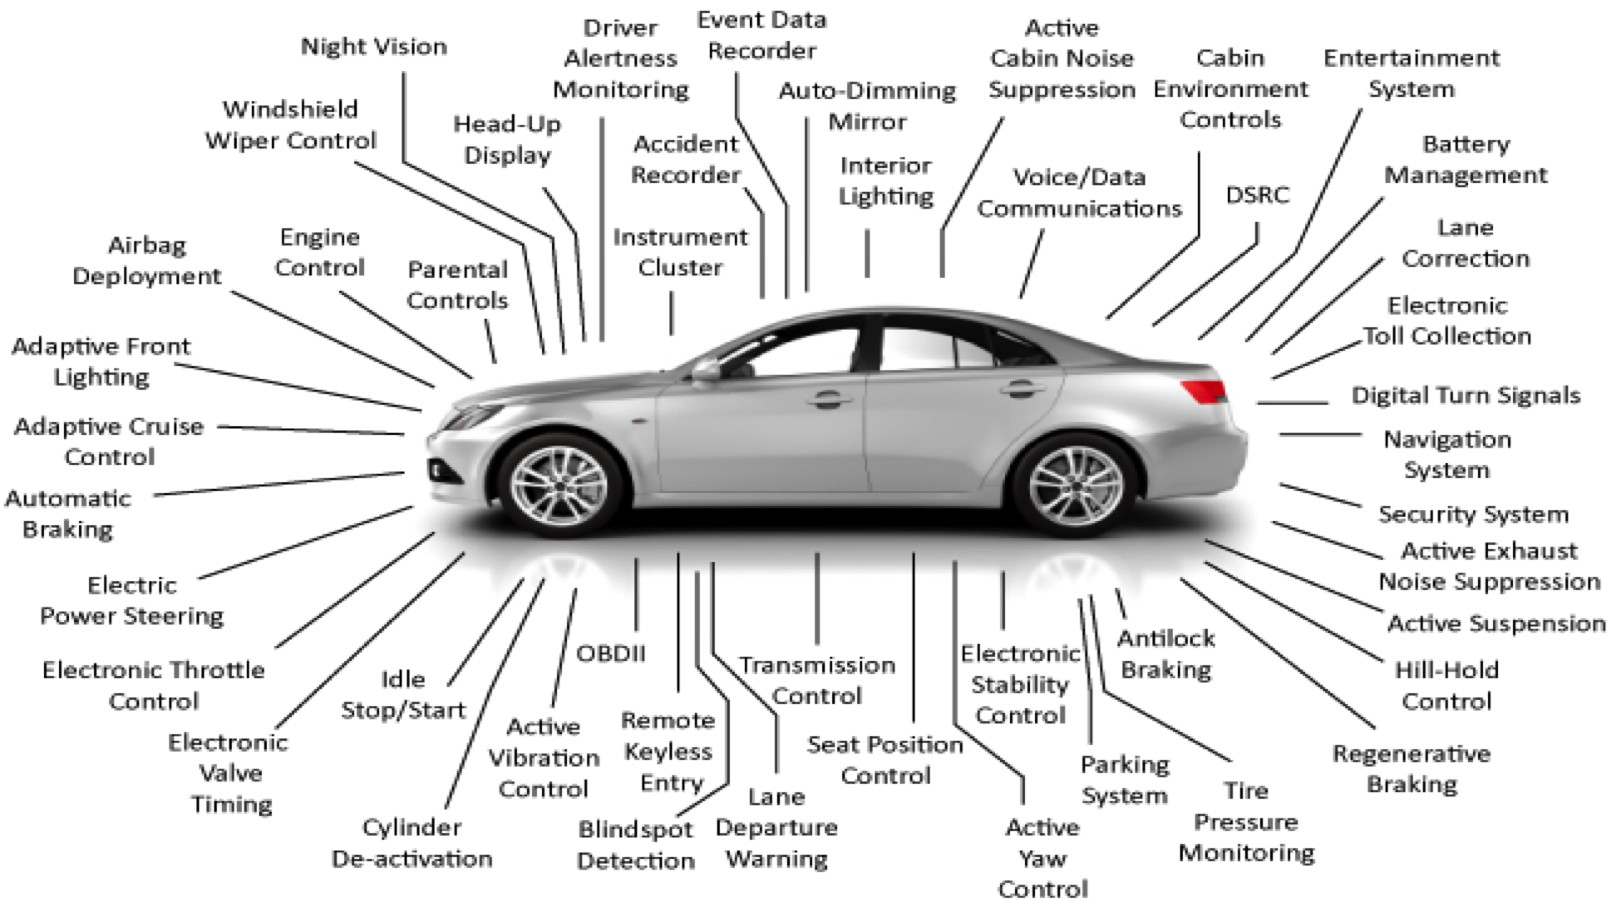
\includegraphics[width=0.85\textwidth]{Images/Diagnostic-Scanning-1.jpg}
    \caption{Mögliche Systemkomponenten, welche durch eine Ransomware missbraucht werden könnten
    \cite{SnapEDABlog.2014}}
    \label{fig:Erpressung}
\end{figure}

\newpage
Abbildung \ref{fig:Erpressung} macht deutlich, dass es in heutigen Autos zahlreiche Systeme gibt, 
auf denen man einen Cyber-Angriff durchführen kann. Sei es das Blockieren wichtiger 
Steuergerätfunktionen oder kryptografischer Anmeldeinformationen, das Verschlüsseln 
von kritischen Daten, das Freigeben kritischer interner Daten im Fahrzeug, das 
Manipulieren von Sensor-/Servodaten oder das Manipulieren bzw. Zerstören kritischer 
Fahrzeugkomponenten – ein Angreifer hat viele Möglichkeiten. 
\newline
Sobald die Geiselnahme durchgeführt oder vorgetäuscht wurde, wird die Ransomware 
für das Opfer sichtbar. Eine solche Erpressungsmeldung erklärt in der Regel die eigentliche 
Erpressungssituation klar und deutlich und gibt sehr detaillierte Anweisungen und Informationen, 
wie das geforderte Lösegeld zu zahlen ist. Zur Demonstration haben die Autoren eine 
solche Meldung erstellt, welche in Abbildung \ref{fig:WannaDrive} zu sehen ist. 
\newline

\begin{figure}[htbp!]
    \centering
    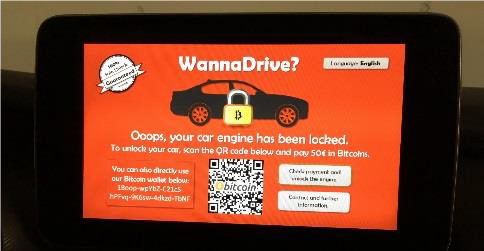
\includegraphics[width=0.75\textwidth]{Images/WannaDrive.png}
    \caption{Beispielhafte Erpressungsmeldung mit Zahlungsinformationen
    \cite{M.Wolf.2017}}
    \label{fig:WannaDrive}
\end{figure}
